\documentclass[12pt]{standalone}
\usepackage{tikz}
\usetikzlibrary{decorations.pathreplacing}
\usetikzlibrary{decorations.markings}
\usetikzlibrary{positioning}
\usetikzlibrary{shapes}
\usetikzlibrary{calc}

\usetikzlibrary{backgrounds}

\begin{document}
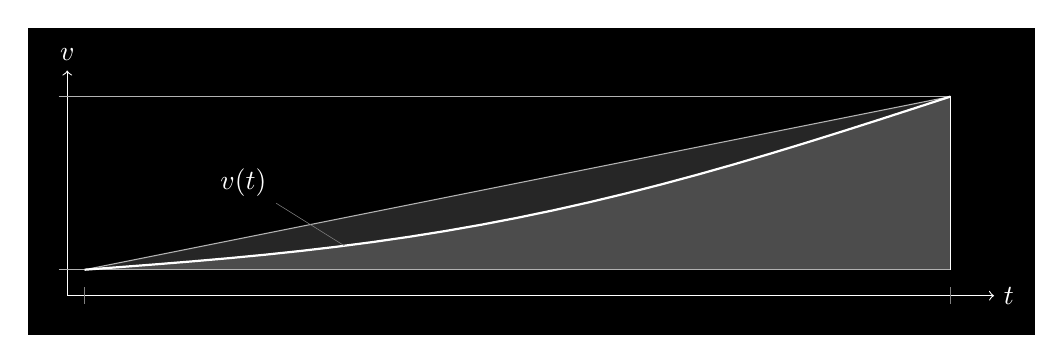
\begin{tikzpicture}[
	scale=11,
	pin distance=10mm,
	pin position=150,
	color=white,
	background rectangle/.style={fill=black},
	show background rectangle]

\IfStandalone {\tikzstyle{subtle}=[thin,gray]
\tikzstyle{subtle line}=[thin,gray!60]} {\tikzstyle{subtle}=[thin,gray]
\tikzstyle{subtle line}=[thin,gray!60]}

\def\XOffset{-0.02}
\def\YOffset{0.03}
\def\LinearCoef{0.2}
\def\NonlinearCoef{-0.04}
\pgfmathsetmacro{\InitialTempo}{\YOffset}
\pgfmathsetmacro{\TargetTempo}{\YOffset + \LinearCoef}
\pgfmathsetmacro{\PlotHeigth}{2 * \YOffset + \LinearCoef}
\pgfmathsetmacro{\CenterTempo}{\YOffset + 0.5 * \LinearCoef}

\begin{scope}[declare function={
	tempo(\t) = \YOffset + \LinearCoef * \t + \NonlinearCoef * sin(pi * \t r);
	}]

% Draw axes
\draw [<->] (\XOffset, \PlotHeigth) node (yaxis) [above] {$v$}
	|- (1.05,0) node (xaxis) [right] {$t$};

% ticks on time axis
\draw[subtle] (0,0.01) -- (0,-0.01) node [below] {};
\draw[subtle] (1,0.01) -- (1,-0.01) node [below] {};

% non-linear position change
\path[fill=black!85]
	(0, \InitialTempo)
	-- (1, \TargetTempo)
	-- (1, \InitialTempo)
	-- cycle;
\node at (0.5, 0.85 * \CenterTempo) [coordinate,
	] {};

% Total position change
\path[fill=black!70,domain=0:1]
	(0, \InitialTempo) --
	plot (\x, { tempo(\x) }) --
	(1, \InitialTempo) --
	cycle;
\node at (0.85, 0.8 * \CenterTempo) {};

% line for linear tempo change
\draw[subtle line]
(0, \InitialTempo) --
(1, \TargetTempo);

% Initial tempo
\draw[subtle line]
(\XOffset - 0.01, \InitialTempo) node[left, subtle] {} -|
(1, \InitialTempo);

% Target tempo
\draw[subtle line]
(\XOffset - 0.01, \TargetTempo) node[left, subtle] {} -|
(1, \TargetTempo);

% Tempo change
\draw [yshift=0pt]
	(1, \InitialTempo) -- (1, \TargetTempo)
	node [black,midway,xshift=0.6cm] {};

% actual function
\draw[thick,domain=0:1] plot (\x, { tempo(\x) });
\node at (0.3, {tempo(0.3)}) [coordinate,
	pin=$v(t)$] {};

\end{scope}
\end{tikzpicture}
\end{document}